\documentclass[english, xcolor=dvipsnames, aspectratio=169]{beamer}
% packages
%----------------------------------------------------------------------------------------
%	PACKAGES AND OTHER DOCUMENT CONFIGURATIONS
%----------------------------------------------------------------------------------------

\documentclass[
	11pt, % Set the default font size, options include: 8pt, 9pt, 10pt, 11pt, 12pt, 14pt, 17pt, 20pt
	%t, % Uncomment to vertically align all slide content to the top of the slide, rather than the default centered
	%aspectratio=169, % Uncomment to set the aspect ratio to a 16:9 ratio which matches the aspect ratio of 1080p and 4K screens and projectors
]{beamer}

\graphicspath{{../../imgs/}{{../../imgs/04_Classification}}} % Specifies where to look for included images (trailing slash required)

\usepackage{booktabs} % Allows the use of \toprule, \midrule and \bottomrule for better rules in tables

\usepackage[T1]{fontenc}
\usepackage{mathptmx}
% Define colors variables
% Define colors variables
\definecolor{red}{rgb}{0.631, 0.094, 0.094} % primary color
\definecolor{grey}{rgb}{0.3686, 0.5255, 0.6235} % secondary color
\definecolor{blue}{rgb}{0.27, 0.509, 0.705} % primary color

% Title page
\title{Neural networks}
\author{Blanca Cano Camarero}
\institute{Universidad Autónoma de Madrid}

  % logo of my university
  \titlegraphic{
    
\includegraphics[width=0.4\textwidth]{logos/uam-iic.jpeg}
}

% Date
\day=16\relax
\month=12\relax
\year=2022\relax

% Color template 
\newcommand{\bgcolor}{blue}
% Beamer parameters
% Set theme palette colors
\setbeamercolor{palette primary}{bg=\bgcolor,fg=white}
\setbeamercolor{palette secondary}{bg=\bgcolor,fg=white}
\setbeamercolor{palette tertiary}{bg=\bgcolor,fg=white}
\setbeamercolor{palette quaternary}{bg=\bgcolor,fg=white}
% strucure means itemize, enumerate, etc
\setbeamercolor{structure}{fg=\bgcolor} 

% Set bibliography colors
\setbeamercolor{bibliography item}{fg=\bgcolor}
\setbeamercolor{bibliography entry author}{fg=black}
\setbeamercolor{bibliography entry title}{fg=black}
\setbeamercolor{bibliography entry location}{fg=black}
\setbeamercolor{bibliography entry note}{fg=black}
% Replaces book icon in bibliography with enumeration
\setbeamertemplate{bibliography item}{[\theenumiv]}

% Table of contents style
% \setbeamertemplate{section in toc}[sections numbe\bgcolor]
% \setbeamertemplate{subsection in toc}[subsections numbe\bgcolor]
\setbeamertemplate{section in toc}[circle]
\setbeamertemplate{subsection in toc}[ball unnumbe\bgcolor]

% Header with navigation bar
\setbeamertemplate{headline}
{
    \leavevmode
    \hbox{
    \begin{beamercolorbox}[wd=\paperwidth,ht=2.5ex,dp=1.125ex]{palette quaternary}
    \insertsectionnavigationhorizontal{\paperwidth}{}{\hskip0pt plus1filll}
    \end{beamercolorbox} 
    }
}
% Footer with custom caption
\setbeamertemplate{footline}
{
    \leavevmode
    \hbox{
    \begin{beamercolorbox}[wd=.33\paperwidth,ht=2.6ex,dp=1ex,center]{palette quaternary}
    \usebeamerfont{author in head/foot}\insertshortauthor\hspace*{1ex}
    \end{beamercolorbox}
    \begin{beamercolorbox}[wd=.33\paperwidth,ht=2.6ex,dp=1ex,center]{palette quaternary}
    \usebeamerfont{institute in head/foot}\insertshortinstitute
    \end{beamercolorbox}
    \begin{beamercolorbox}[wd=.33\paperwidth,ht=2.6ex,dp=1ex,center]{palette quaternary}
    \insertframenumber{} / \inserttotalframenumber
    \end{beamercolorbox}}
    \vskip0pt
}

%% Custom commands
%% ===============

%% Special characters for number sets, e.g. real or complex numbers.
\newcommand{\C}{\mathbb{C}}
\newcommand{\K}{\mathbb{K}}
\newcommand{\N}{\mathbb{N}}
\newcommand{\Q}{\mathbb{Q}}
\newcommand{\R}{\mathbb{R}}
\newcommand{\Z}{\mathbb{Z}}
\newcommand{\X}{\mathbb{X}}

%% Fixed/scaling delimiter examples (see mathtools documentation)
\DeclarePairedDelimiter\abs{\lvert}{\rvert}
\DeclarePairedDelimiter\norm{\lVert}{\rVert}

%% Use the alternative epsilon per default and define the old one as \oldepsilon
\let\oldepsilon\epsilon
\renewcommand{\epsilon}{\ensuremath\varepsilon}

%% Also set the alternate phi as default.
\let\oldphi\phi
\renewcommand{\phi}{\ensuremath{\varphi}}

\newcommand{\logo}[1][\textwidth]{\resizebox{#1}{!}{
\includegraphics{logos/uam-iic.jpeg}}}




\begin{document}

\frame{\titlepage}

% Complete table of contents (ToC)
% \customToC{hideallsubsections}{}
%\customToC{}{}

%%%%%%% add sections here %%%%%%%
% Section name and highlighted ToC
%\renewcommand{\sectiontitle}{Introduction}
%\section{\sectiontitle}
%\customToC{currentsection,hideothersubsections}{}

% Section name and highlighted ToC
%\renewcommand{\subsectiontitle}{What is machine learning?}
%\subsection{\subsectiontitle}


\begin{frame}{Overview}
  \tableofcontents
\end{frame}
%%%% Work summary 
\section{Article data}

\begin{frame}
    \frametitle{Understanding the difficulty of training deep feedforward neural networks}
      \begin{itemize}
        \item Authors: Xavier Glorot and Yoshua Bengio.
        \item Publication year: 2010.
        \item Conference: Proceedings of the thirteenth international conference on artificial intelligence and statistics.
        \item Cited by: 19886 (I have found is quite a lot!) 
      \end{itemize}
      Reference: \cite{Understanding_the_difficulty_of_training_deep_feedforward_neural_networks}
\end{frame}

\section{Abstract}
\begin{frame}
  \frametitle{Abstract}

  \textbf{Context}
  \begin{itemize}
    \item Before 2006 deep multilayer neural networks were not successfully trained. 
    \item But after, by new initialization or training mechanisms experimental results showed the superiority of deeper vs less deep architectures. 
  \end{itemize}

  \textbf{Article objetive}
  \begin{itemize}
    \item Understand why standard gradient descent from random initialization is doing so poorly with deep neural networks. 
  \end{itemize}

  %\textbf{Motivation}
 % \begin{itemize}
  %  \item Design better algorithm. 
  %\end{itemize}
  
\end{frame}
    
\begin{frame}
  
  \textbf{Experiments}
  \begin{itemize}
    \item Observe the influence of the non-linear activations functions:
    \begin{itemize}
      \item Logistic sigmoid activation is unsuited for deep networks for deep networks with random initialization due to its mean value, which can drive especially the \textbf{top hidden layer into saturation}. 
      \item Saturated units can move out of saturation by themselves, albeit slowly (and explain the plateaus sometimes seen when training neural networks). 
      \item Found a new non-linearity that saturares less can often be beneficial. 
  \end{itemize}
    \item They \textbf{study how activations and gradients vary across layers and during training}, with the idea that training may be more difficult when the singular values of the Jacobian associated with each layer are far from one. 
    \item They proposed a new initialization scheme that brings substantially faster convergence. 
  \end{itemize}
  
\end{frame}

\section{Art state}

\begin{frame}
  \frametitle{Art state}

\end{frame}

\section{Experimental setting and Datasets}
\begin{frame}
  \frametitle{Experimental setting and Datasets}
   \textbf{Online learning on a synthetic images dataset: \textbf{Shapeset- 3} $\times 2$ dataset.}
  \begin{itemize}
    \item Focus on optimization issues rather than on the small-sample regularization effects.
    \item  The learner tries to predict which objects (parallelogram, triangle, or elipse) are presented, and one or two objects can be present yield into 9 possible classification.  
  \end{itemize}

  \begin{figure}[t]
    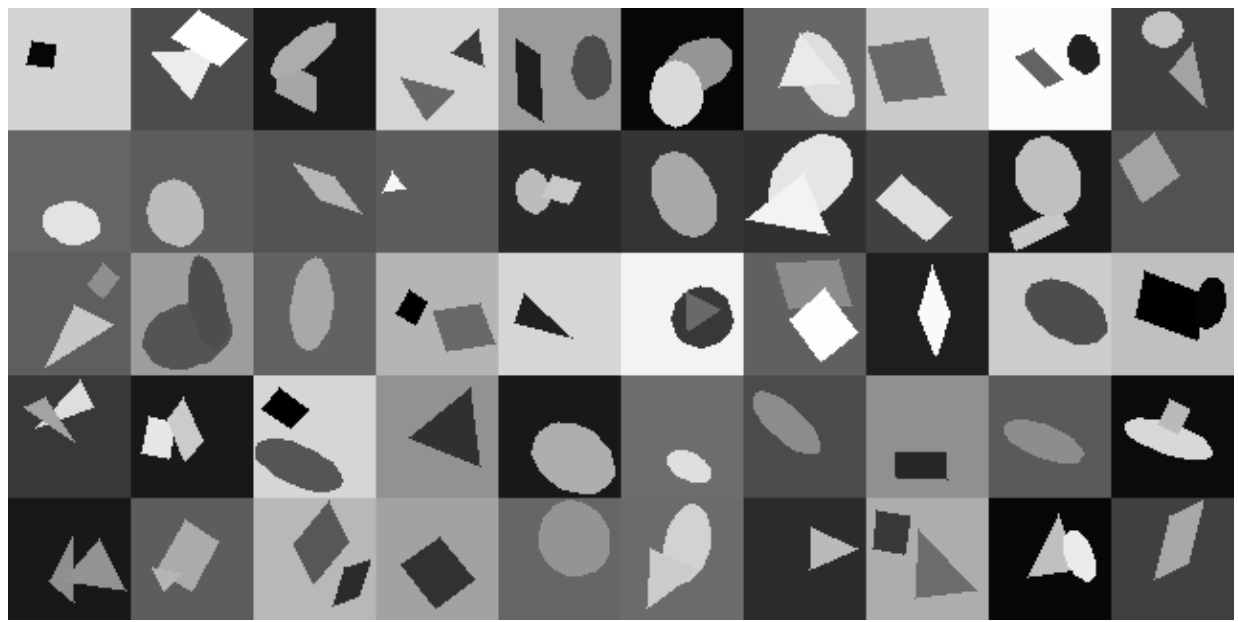
\includegraphics[height=0.4\textheight]{05_Understanding_deep_learning/shapeset-3x2.png}
    \centering
\end{figure}

\end{frame}

\begin{frame}
  \frametitle{Finite Datasets}

  \begin{itemize}
    \item The MNIST digits. 
    \begin{itemize}
      \item 50,000 training images,
      \item 10,000 validations images.
    \end{itemize}
    \item CIFAR-10 labeled subset of the tiny images. 
    \begin{itemize}
      \item 50,000 training images,
      \item 10,000 validations images,
      \item 10 classes corresponding to he main object:  airplane, au- tomobile, bird, cat, deer, dog, frog, horse, ship, or truck.
      \item Classes are balanced. 
    \end{itemize}

    \item Small-ImageNet. 
   \begin{itemize}
      \item 90,000 training images,
      \item 10,000 validations images,
      \item 10 classes corresponding to he main object: reptiles, vehicles, birds, mammals, fish, furniture, instruments, tools, flowers and fruits.
      \item Classes are balanced. 
    \end{itemize}
  \end{itemize}

\end{frame}

\begin{frame}
  \begin{figure}
    \centering
    \begin{subfigure}[b]{0.3\textwidth}
        \centering
        
\includegraphics[width=\textwidth]{05_Understanding_deep_learning/MNIST.png}
        \caption{MNIST}
        \label{fig:y equals x}
    \end{subfigure}
    \hfill
    \begin{subfigure}[b]{0.3\textwidth}
        \centering
        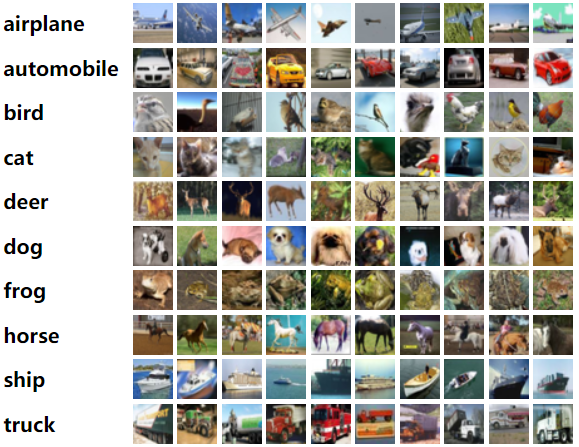
\includegraphics[width=\textwidth]{05_Understanding_deep_learning/CIFAR-10.png}
        \caption{CIFAR-10}
        \label{fig:three sin x}
    \end{subfigure}
    \hfill
    \begin{subfigure}[b]{0.3\textwidth}
        \centering
        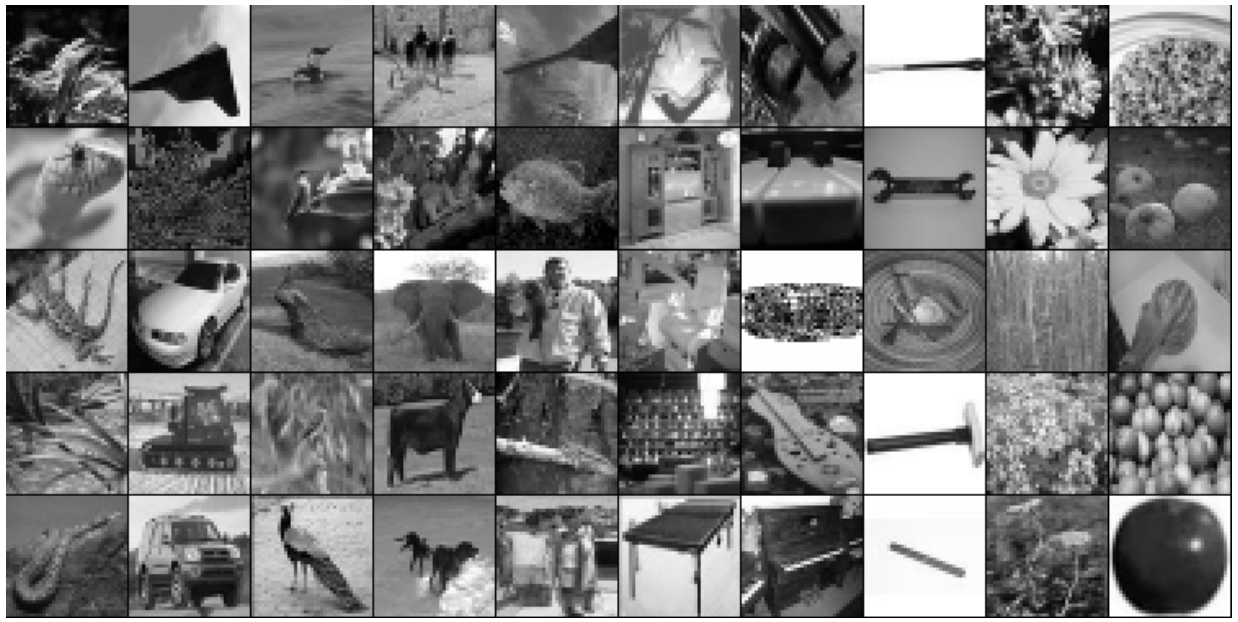
\includegraphics[width=\textwidth]{05_Understanding_deep_learning/small-ImageNet.png}
        \caption{Small-ImageNet}
        \label{fig:five over x}
    \end{subfigure}
       \caption{Three simple graphs}
       \label{fig:three graphs}
\end{figure}
\end{frame}

\begin{frame}
  \frametitle{Experimental Setting}
  \begin{itemize}
    \item They optimized feedforward neural networks: 
    \begin{itemize}
      \item With one to five hidden layers. 
      \item One thousand hidden units per layer. 
      \item Softmax logistic regression for the output. 
    \end{itemize}
    \item Cost function is the negative log-likelihood: 
    \begin{equation}
      - \log P(y|x),
    \end{equation}
    where $(x,y)$ is the (input image, target class). 
    \item NN optimized with stochastic back-propagation on mini-batches of size ten. 
    \item Learning rate is a hyperparameter that is optimized based on validation set error after a large number of updates (5 million). 
  \end{itemize}
\end{frame}

\begin{frame}
  \frametitle{Experimental setting}

  \begin{itemize}
    \item The non-linear activation functions in the hidden layers varied on: 
    \begin{itemize}
      \item The sigmoid
      \item the hyperbolic tangent,
      \item the \textit{newly proposed} softsign: 
      \begin{equation}
        \frac{x}{1 + |x|}
      \end{equation}
    \end{itemize}
  \end{itemize}

  \begin{figure}[t]
    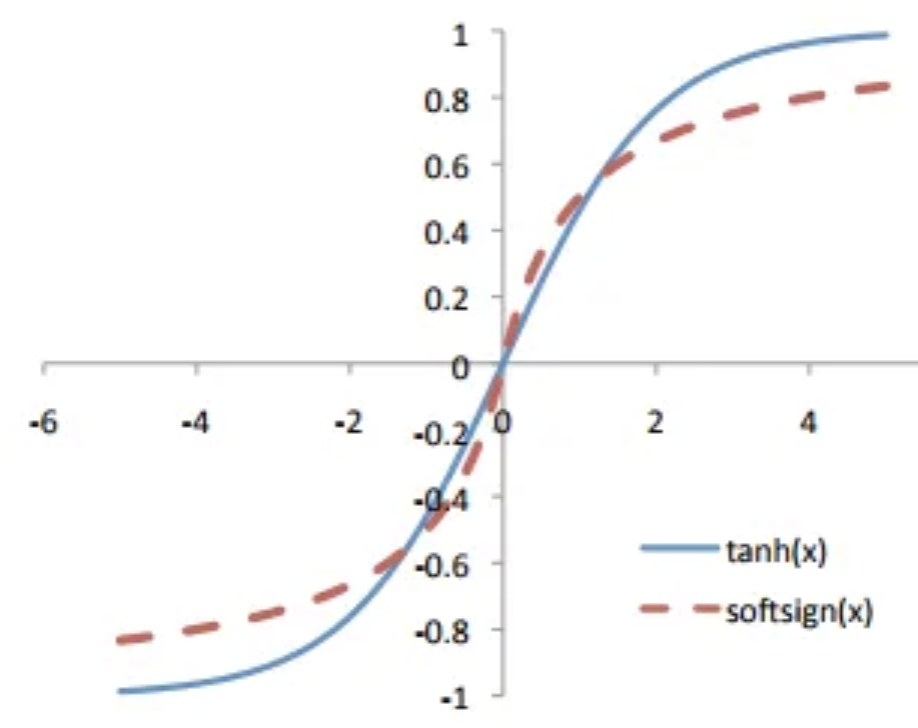
\includegraphics[height=0.4\textheight]{05_Understanding_deep_learning/softsign.png}
    \centering
\end{figure}

\end{frame}

\begin{frame}
  \frametitle{Experimental setting}

  \begin{itemize}
    \item They search for the best hyperparameters (learning rate and depth) separately for each model. 
    \item Initialization: 
    \begin{itemize}
      \item Biases to 0,
      \item the weight $W_{i j}$ at each layer with the following commonly used heuristic 
      \begin{equation}
        W_{i j} \sim U \left( - \frac{1}{\sqrt{n}}, \frac{1}{\sqrt{n}}\right), 
      \end{equation}
      where $U$ is the uniform distribution and $n$ the size of the previous layer. 
    \end{itemize}
  \end{itemize}

\end{frame}

\section{Effect of Activation Functions and Saturation During Training}

\begin{frame}
  \frametitle{Avoidable things}
\begin{itemize}
  \item Excessive saturation of activation functions (affects gradient propagation). 
  \item Overlay linear units  (will not compute something interesting).
\end{itemize}
\end{frame}

\subsection{Experiments with the Sigmoid}
\begin{frame}
  \frametitle{Experiments with the Sigmoid}

    The sigmoid non-linearity has symptomatic behaviour.
    
    \begin{itemize}
      \item Its none-zero mean that induces import singular values in the Hessian. 
      \item Saturation levels. 
    \end{itemize} 

    \textbf{Experiments considerations}

    \begin{itemize}
      \item looking at the evolution of activations during training on the Shapeset-3 x 2 data.
      
      \item  Figure \ref{fig:saturation-sigmoid-shapeset3x2} shows the evolution of the activation values (after the non- linearity) at each hidden layer during training of a deep architecture with sigmoid activation functions. 
      
      \item Layer 1 refers to the output of first hidden layer, and there are four hidden layers. 
      
      \item The graph shows the means and standard deviations of these activations. 
      
      \item These statistics along with histograms are computed at different times during learning, by looking at activation values for a fixed set of 300 test examples. 
    \end{itemize}
\end{frame}

\begin{frame}
  \frametitle{Evolution ot the activations during training}
% imgs/05_Understanding_deep_learning/saturation_sigmoid.png
\begin{figure}[t]
  \centering
  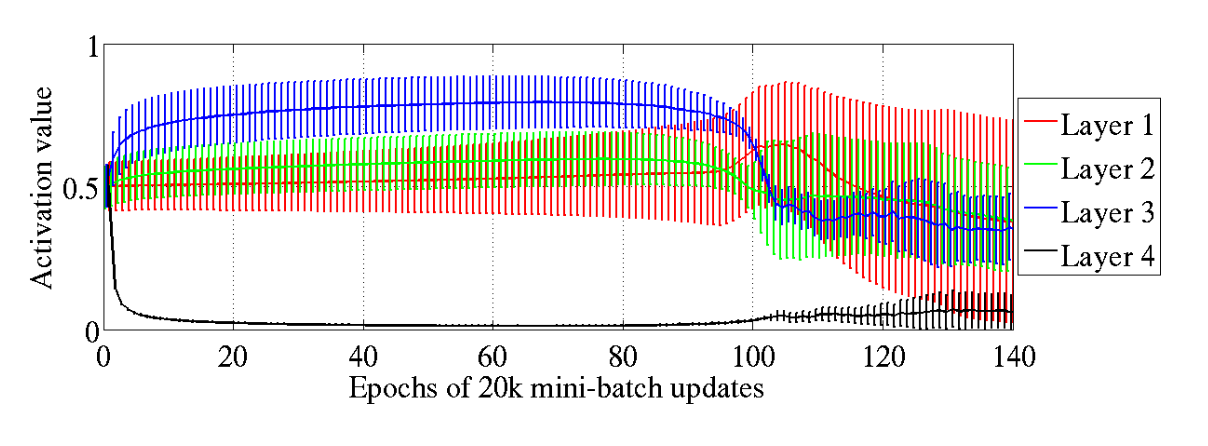
\includegraphics[height=0.6\textheight]{05_Understanding_deep_learning/saturation_sigmoid.png}
  \caption{Mean and standard deviation (vertical bars) of the activation values (output of the sigmoid) during supervised learning, for the different hidden layers of a deep architecture. The top hidden layer quickly saturates at 0 (slow- ing down all learning), but then slowly desaturates around epoch 100.}
  \label{fig:saturation-sigmoid-shapeset3x2}
\end{figure}

\end{frame}

\begin{frame}
  \frametitle{Observation}

  \begin{itemize}
    \item We see that very quickly at the beginning, all the sigmoid activation values of the last hidden layer are pushed to their lower saturation value of 0.
    
    \item the others layers have a mean activation value that is above 0.5, and decreasing as we go from the output layer to the input layer. 
    
    \item This kind of saturation can last very long in deeper networks with sigmoid activations, e.g., the depth-five model never escaped this regime during training. 
    
    \item The big surprise is that for intermediate number of hidden layers (here four), the saturation regime may be escaped. 
    
    \item The top hidden layer moves out of saturation, the first hidden layer begins to saturate and therefore to stabilize.

  \end{itemize}

\end{frame}

\begin{frame}
  \frametitle{Hypothesis}

  \begin{itemize}
    \item This behavior is due to the combination of \textbf{random initialization} and the fact that an hidden \textbf{unit output of 0 corresponds to a saturated} sigmoid since  deep networks with sigmoids but initialized from unsupervised pre-training (e.g. from RBMs) do not suffer from this saturation behavior.
    
    \item  the lower layers of the randomly initialized network computes initially is not useful to the classification task, unlike the transformation obtained from unsupervised pre-training.
    
    \item The logistic layer output $softmax(b + W h)$ might initially rely more on its biases b (which are learned very quickly) than on the top hidden activations $h$ derived from the input image (because $h$ would vary in ways that are not predictive of $y$). 
  \end{itemize}

\end{frame}


\begin{frame}
  \frametitle{Hypothesis}

  \begin{itemize}
    \item Would the error gradient wold tend to push $Wh$ towards 0, which can be achieved by pushing $h$ towards $0$. 
    
    \item  Symmetric activation functions like the hyperbolic tangent and the softsign, sitting around 0 is good because it allows gradients to flow backwards.
    
    \item pushing the sigmoid outputs to 0 would bring them into a saturation regime which would prevent gradients to flow backward and prevent the lower layers from learning useful features. 
    
    \item Eventually but slowly, the lower layers move toward more useful features and the top hidden layer then moves out of the saturation regime. However that, even after this, the network moves into a solution that is of poorer quality 
  \end{itemize}

\end{frame}


\begin{frame}
  \frametitle{Test error during online training}

  % imgs/05_Understanding_deep_learning/test_error_during_online_training.png
  \begin{figure}[t]
    \centering
    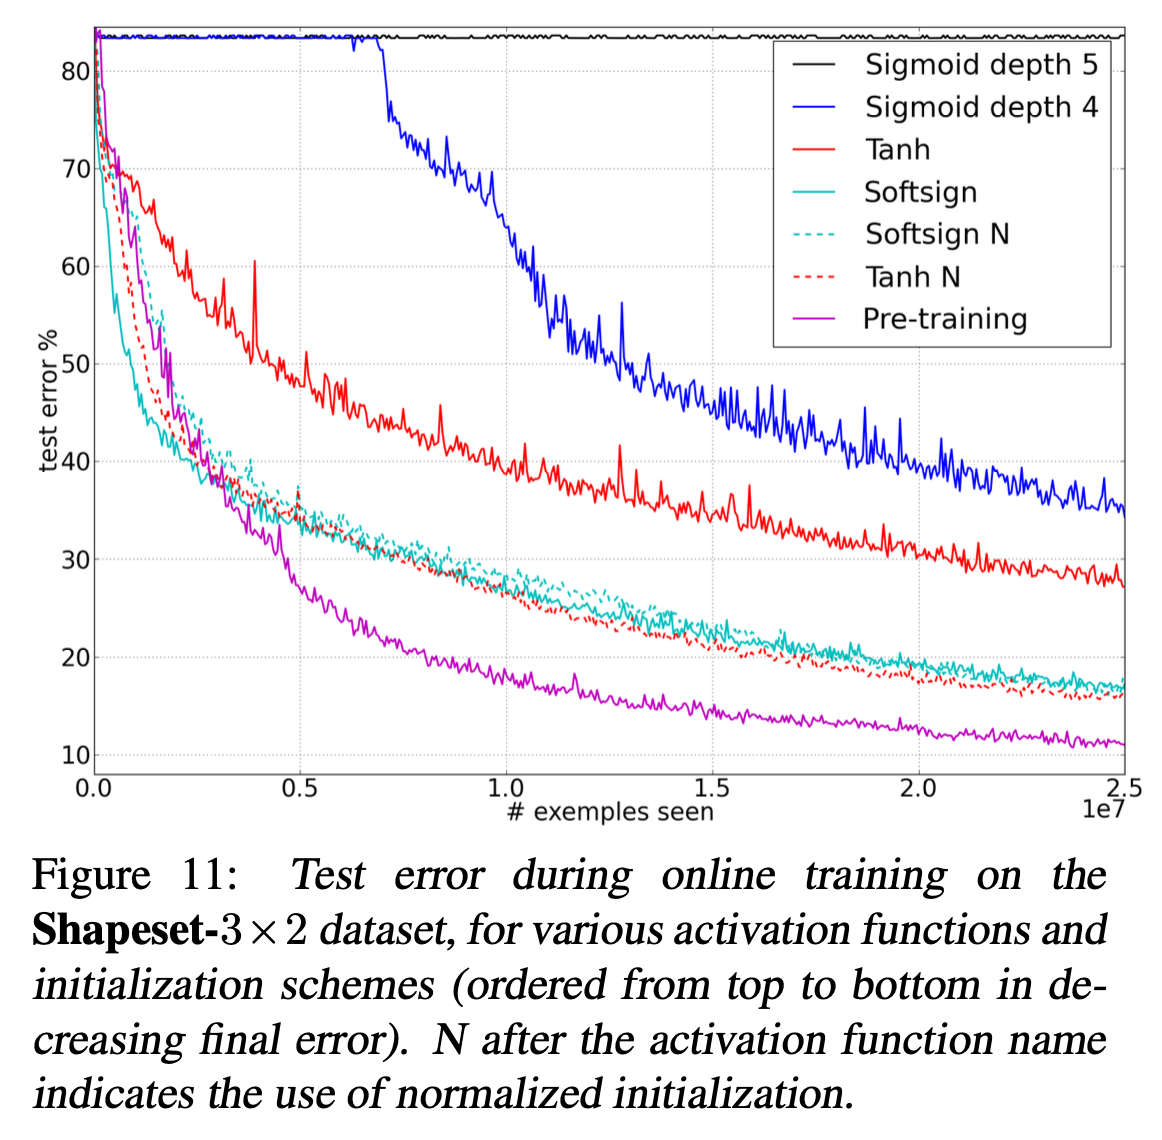
\includegraphics[height=0.8\textheight]{05_Understanding_deep_learning/test_error_during_online_training.png}
  \end{figure}
\end{frame}


\subsection{Experiments with the Hyperbolic tangent}

\begin{frame}
  \frametitle{Experiments with the Hyperbolic tangent}

  \begin{itemize}
    \item The hyperbolic tangent networks do not suffer from the kind of saturation behavior of the top hid- den layer observed with sigmoid networks, because of its symmetry around 0.
    \item With the standard weight initialization, we observe a sequentially occurring saturation phenomenon starting with layer 1 and propagating up in the network, as illustrated in Figure 3. 
    \item \textbf{Why this is happening remains to be understood.}

  \end{itemize}

\end{frame}


\begin{frame}
  \frametitle{Activation values for hiperbolic tangent and softsign}

  % imgs/05_Understanding_deep_learning/distribution_of_activation_values_for_the_hyperbolic_and_soft_sign.png
  \begin{figure}[t]
    \centering
    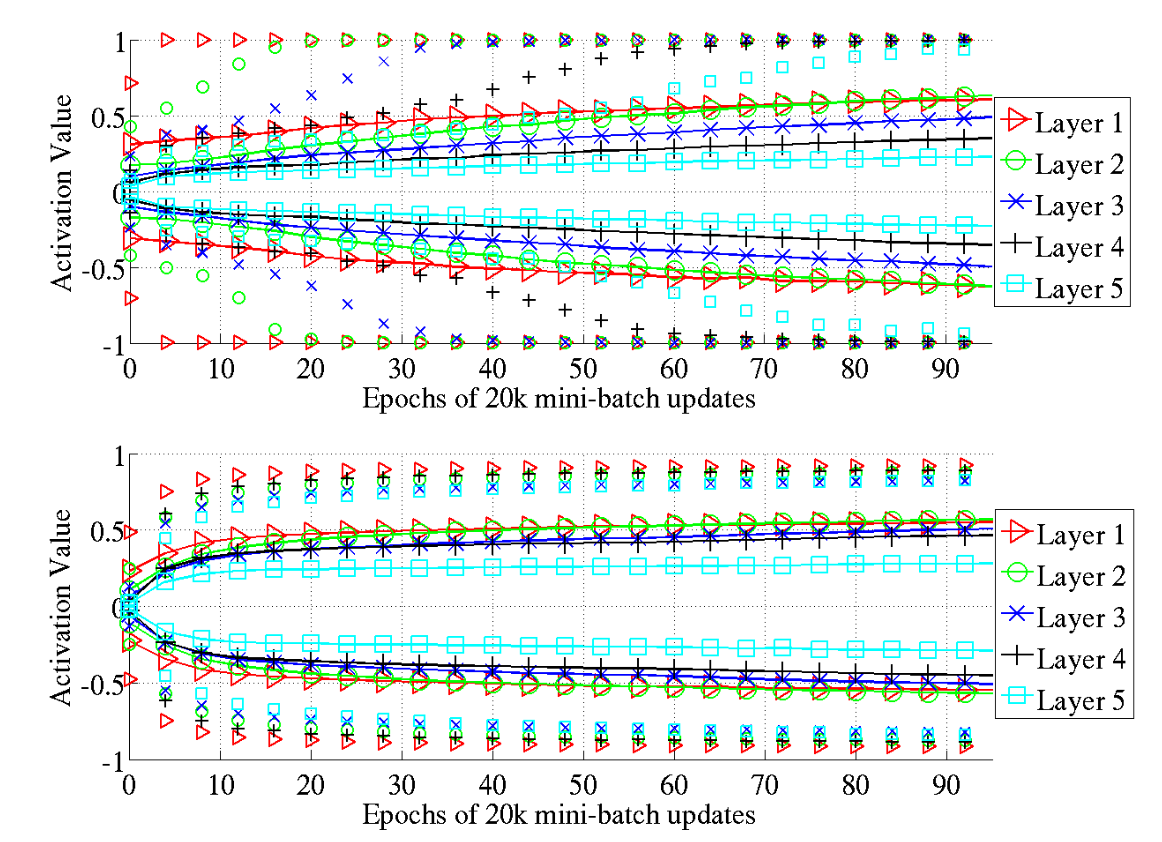
\includegraphics[height=0.5\textheight]{05_Understanding_deep_learning/distribution_of_activation_values_for_the_hyperbolic_and_soft_sign.png}
    \caption{
      Top:98 percentiles (markers alone) and standard deviation (solid lines with markers) of the distribution of the activation values for the hyperbolic tangent networks in the course of learning. We see the first hidden layer satu- rating first, then the second, etc. Bottom: 98 percentiles (markers alone) and standard deviation (solid lines with markers) of the distribution of activation values for the soft- sign during learning. Here the different layers saturate less and do so together.
    }
  \end{figure}

\end{frame}

\subsection{Experiments with the Softsign}


\begin{frame}
  \frametitle{Experiments with the Softsign}

  \begin{itemize}
    \item The softsign $x/(1+|x|)$ is similar to the hyperbolic tangent but might behave differently in terms of saturation because of its smoother asymptotes (polynomial instead of exponential). 
    
    \item We see on Figure 3 that the saturation does not occur one layer after the other like for the hyperbolic tangent. It is faster at the beginning and then slow, and all layers move together towards larger weights.
  \end{itemize}

\end{frame}

\begin{frame}
  \frametitle{Histogram of activation values at the end of the learning}
% imgs/05_Understanding_deep_learning/activation_values_at_end_of_the_learning.png
\begin{figure}[t]
  \centering
  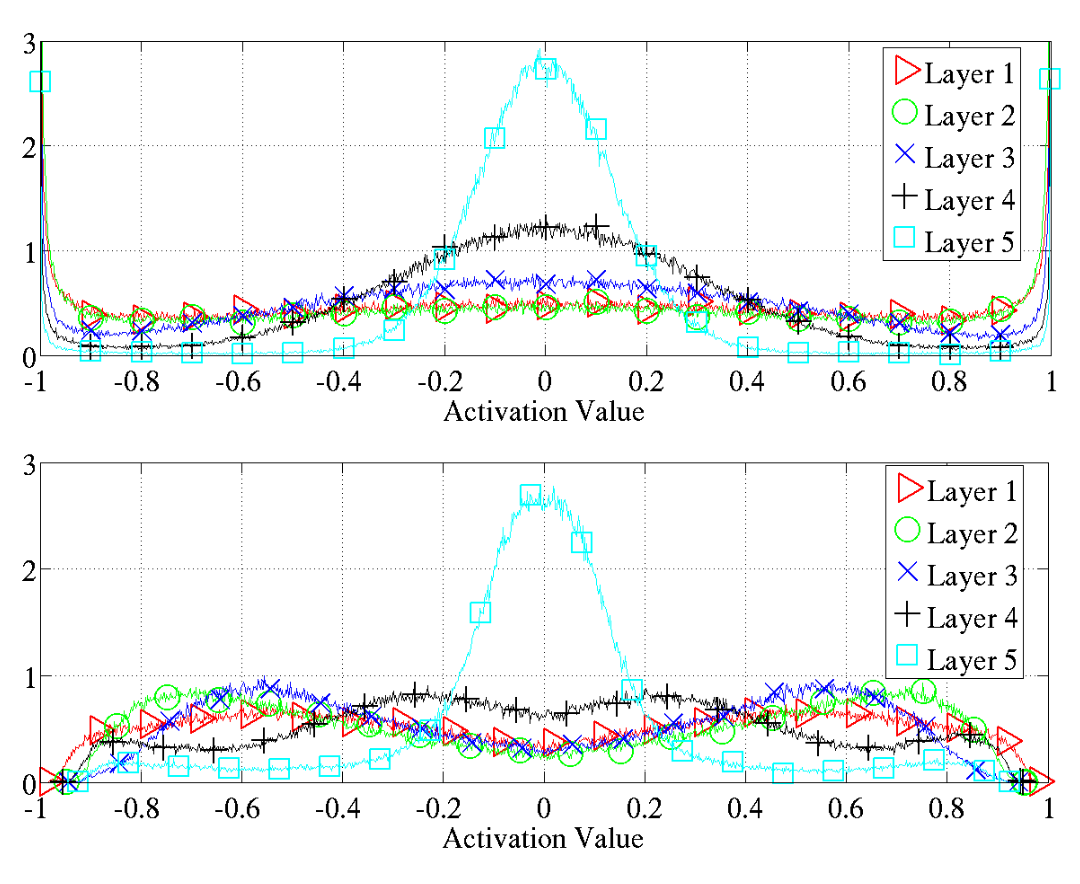
\includegraphics[height=0.5\textheight]{05_Understanding_deep_learning/activation_values_at_end_of_the_learning.png}
  \caption{
    Activation values normalized histogram at the end of learning, averaged across units of the same layer and across 300 test examples. Top: activation function is hyperbolic tangent, we see important saturation of the lower layers. Bottom: activation function is softsign, we see many activation values around (-0.6,-0.8) and (0.6,0.8) where the units do not saturate but are non-linear.
  }
\end{figure}
  
\end{frame}

\section{Studying Gradients and their Propagation}


    
\section{Network Training}

\begin{frame}
  \frametitle{The error function}


\begin{equation}
  t = y(x,w) + \epsilon 
\end{equation}
where $\epsilon \sim \mathcal{N}(0, \beta^{-1})$ 
and $\beta \in \R$ is the precision ($\beta^{-1} = \sigma^2$). 

Thus we can write
% la probabilidad t a partir de x es 
%  igual a la probabilidad de que t lo sea a partir de la normal
% abuso de notación N
% N es la función de probabilidad de una normal 
% de media y y de varianza la inversa de la precisión 
\begin{equation}
  p(t | x, w, \beta) = \mathcal{N}(t | y(x,w), \beta^{-1}). 
\end{equation}

\end{frame}


\begin{frame}
  For a single real-valued variable x, the Gaussian distribution is defined by

  \begin{equation}
    \mathcal{N}(x | \mu, \sigma^2) 
    = 
    \frac{1}{\sqrt{2 \pi \sigma^2}}
    \exp 
    \left\{
      - \frac{1}{2 \sigma^2} (x - \mu)^2
    \right\}. 
  \end{equation}

  We have to minimize the following error function
  \begin{equation}
    - \log p(t|X,w, \beta) 
    =
    \frac{n \beta}{2} 
    \sum_{i = 1}^n
    \left\{
      y(x_i, w)
      -
      t_i
    \right\}^2
    - 
    % first fraction 
    \frac{n}{2} \log \beta 
    - \frac{n}{2} \log(2 \pi) 
  \end{equation}
  which can be used to learn the parameters 
  $w$ and $\beta$. 
\end{frame}


\begin{frame}
  \frametitle{The error function}

  Let take the error function as the 
  \begin{equation}
    E(w)
    = 
    \frac{1}{2} 
    \sum_{i = 1}^n
    \left\{
      y(x_i, w)
      -
      t_i
    \right\}^2
  \end{equation}
  where we have discarded additive and multiplicative constant.

  Some considerations: 
  \begin{itemize}
    \item The value of $w$ found by minimizing $E(w)$ will be denoted as $w_{ML}$ (maximum likelihood solution).
    \item The nonlinearity of the network function $y(x_n, w)$ causes the error $E(w)$ to be nonconvex.
    \item So in practice $W_{ML}$ would be a local minimum. 
  \end{itemize}
\end{frame}

\begin{frame}
  \frametitle{About the precision}

  Having found $w_{ML}$ the value of $\beta$ can be found by minimizing the negative log likelihood to give 

  \begin{equation}
    \frac{1}{\beta_{ML}}
    = 
    \frac{1}{N}
    \frac{1}{2} 
    \sum_{i = 1}^N
    \left\{
      y(x_i, w_{ML})
      -
      t_i
    \right\}^2
  \end{equation}

\end{frame}

\begin{frame}
  \frametitle{Multiple target variable}

  \begin{equation}
    p(t | x, w)
    = 
    \mathcal{N}(t | y(x,w), \beta^{-1} I). 
  \end{equation}

  The noise precision is the given by 
  \begin{equation}
    \frac{1}{\beta_{ML}}
    = 
    \frac{1}{N K}
    \sum_{i = 1}^N
    \|
    y(x_i, w_{ML}) - t_i
    \|^2
  \end{equation}
\end{frame}

\begin{frame}
  \frametitle{Minimizing regression case}
\begin{equation}
  \frac{\partial E}{\partial a_k}
  = y_k  - t_k
\end{equation}
\end{frame}

\begin{frame}
  \frametitle{Binary classification problem}
We have a single target $t$ such that $t = 1$
dentotes class $C_1$ and $t=0$ denotes class
$C_2$. 

As we see last week we consider a single output whose
activation function is a logistic sigmoid: 

\begin{equation}
  y = 
  \frac{1}{1 + exp(-a)}
\end{equation}
so that 
\begin{equation}
  0 
  \leq 
  y(x,w)
  \leq
  1.
\end{equation}
We can interpret $y(x,w)$ as the condicional probability 
$p(C_1 |x)$.
\end{frame}

\begin{frame}
  \frametitle{The cross entropy error function}
  The conditional distribution of targets given 
  inputs is the Bernoulli distribution of the form

  \begin{equation}
    p(t|x,w)
    = 
    y(x,w)^t
    \left\{
      1 - y(x,w)
    \right\}^{1-t}.
  \end{equation}

  If we consider a training set of independent observation, 
  then the error function which is given by the negative log 
  likelihood, is then a cross entropy error function of the form 

  \begin{equation}
    E(w)
    =
    - 
    \sum_{n = 1}^N
    \left\{ 
      t_n \log y_n
      +
      (1-t_n) \log(1 - y_n)
    \right\}
  \end{equation}
Using cross entropy error function instead of the sum of squares 
for classification problem leads to faster training as well as improved generalization.
\end{frame}


\begin{frame}
  \frametitle{K binary classification}

  \begin{equation}
    p(t|x,w)
    = 
    \prod_{k=1}^K
    y(x,w)^t
    \left\{
      1 - y(x,w)
    \right\}^{1-t}.
  \end{equation}

  \begin{equation}
    E(w)
    =
    - 
    \sum_{n = 1}^N
    \sum_{k = 1}^K
    \left\{ 
      t_{n k} \log y_{n k}
      +
      (1-t_{n k}) \log(1 - y_{n k})
    \right\}
  \end{equation}

\end{frame}

\begin{frame}
  \frametitle{1 of K coding scheme}
The network outputs are interpreted as
\begin{equation}
  y_k(x,w)
  = 
  p(t_k = 1 | x),
\end{equation}
leading to the following error function
  \begin{equation}
    E(w)
    = 
    - \sum_{n=1}^N
    \sum_{k=1}^K
    t_{k n}
    \log y_k(x_n, w).
  \end{equation}
\end{frame}

\section{Universal approximator}
\begin{frame}
  \frametitle{Universal approximator}

  This paper rigorously establishes that standard multilayer feedforward networks with as few as one hidden layer using arbitrary squashing functions are capable of approximating any Borel measurable function from one finite dimensional space to another to any desired degree of accuracy, provided sufficiently many hidden units are available. In this sense, multilayer feedforward networks are a class of universal approximators.
  \cite{Multilayerfeedforwardnetworksareuniversalapproximators}

\end{frame}
\section{Backpropagation}
\begin{frame}
  \frametitle{Backpropagation}
\begin{equation}\label{eq:descenso-gradiente}
    h_{t+1}  = h_t - \eta \nabla E(h_t).
\end{equation} 
Properties 
\begin{itemize}
  \item Local optimization. 
  \item Fix the number of neurons first. 
  \item $\eta$ is a hyperparameter.  
\end{itemize}
\end{frame}

\begin{frame}
  \frametitle{Our model}

  \begin{equation}\label{eq:red-neuronal-que-aprender}
    h_k(x) = 
    \sum_{j=1}^n \beta_{j k}
    \sigma
    \left(  
        \alpha_{0 j} +
        \sum_{i=1}^d \alpha_{i j}x_i
    \right)
\end{equation}
  
\end{frame}

\begin{frame}
  \frametitle{Derivative with respect to $\beta_{v w}$ st $v \in \{1, \ldots, n\}$ and $w \in \{1, \ldots, s\}$}
{\tiny
    \begin{align} \label{eq:parcial_beta}
        \frac{\partial E(h)}{\partial \beta_{v w}} 
        = &
        \frac{\partial}{\partial \beta_{v w}}
        \left[
            \frac{1}{2}
            \sum_{(x,y) \in \mathcal{D}}
            \sum_{k = 1}^s 
            \left(h_k(x) - y_k \right)^2
        \right]
        \\ % primer paso regla de la cadena
        = &
        \frac{1}{2}
        \sum_{(x,y) \in \mathcal{D}}
        \sum_{k = 1}^s 
        2 \left(h_k(x) - y_k \right)
        \frac{\partial h_k(x)}{\partial \beta_{v w}} 
        \\ 
        = & % desarrollamos h
        \sum_{(x,y) \in \mathcal{D}}
        \sum_{k = 1}^s 
        \left(h_k(x) - y_k \right)
        \frac{\partial}{\partial \beta_{v w}} 
        \left[
            \sum_{j = 1}^n 
                \beta_{j k}
                \sigma
                \left(  
                    \alpha_{0 j} +
                    \sum_{i=1}^d \alpha_{i j}x_i
                \right)
        \right] 
        \\ 
        = & % parcial de la suma es suma de parciales 
        \sum_{(x,y) \in \mathcal{D}}
        \sum_{k = 1}^s 
        \left(h_k(x) - y_k \right)
        \left(
            \sum_{j = 1}^n 
            \frac{\partial}{\partial \beta_{v w}} 
            \left[
                \beta_{j k}
                \sigma
                \left(  
                    \alpha_{0 j} +
                    \sum_{i=1}^d \alpha_{i j}x_i
                \right)
            \right]
        \right) 
        \\ 
        = & % Expresión a partir de la función caraterísticas
        \sum_{(x,y) \in \mathcal{D}}
        \sum_{k = 1}^s 
        \left(h_k(x) - y_k \right)
        \left(
            \sum_{j = 1}^n 
                \chi_{[j = v \wedge k = w]}
                \sigma
                \left(  
                    \alpha_{0 j} +
                    \sum_{j=1}^d \alpha_{i j}x_i
                \right)
        \right)
        \\ 
        = & % Expresión final quitando términos nulos 
        \sum_{(x,y) \in \mathcal{D}}
        \left(h_w(x) - y_w \right)
        \left(
            \sigma
            \left(  
                \alpha_{0 v} +
                \sum_{i=1}^d \alpha_{i v}x_i
            \right)
        \right).
    \end{align}
  }
\end{frame}

\begin{frame}
  \frametitle{Derivative with respect to $\alpha_{0 v}$ st $v \in \{1, \ldots, n\}$}
  {\tiny 
  \begin{align} \label{eq:parcial_alpha_cero}
        \frac{\partial E(h)}{\partial \alpha_{0 v}} 
        = &
        \frac{\partial}{\partial \alpha_{0 v}}
        \left[
            \frac{1}{2}
            \sum_{(x,y) \in \mathcal{D}}
            \sum_{k = 1}^s 
            \left(h_k(x) - y\right)^2
        \right]
        \\ % primer paso regla de la cadena
        = &
        \frac{1}{2}
        \sum_{(x,y) \in \mathcal{D}}
        \sum_{k = 1}^s 
        2 \left(h_k(x) - y_k \right)
        \frac{\partial h_k(x)}{\partial \alpha_{0 v}} 
        \\ 
        = & % desarrollamos h
        \sum_{(x,y) \in \mathcal{D}}
        \sum_{k = 1}^s 
        \left(h_k(x) - y_k \right)
        \frac{\partial}{\partial \alpha_{0 v}} 
        \left[
            \sum_{j = 1}^n 
                \beta_{j k}
                \sigma
                \left(  
                    \alpha_{0 j} +
                    \sum_{i=1}^d \alpha_{i j}x_i
                \right)
        \right] 
        \\ 
        = & % parcial de la suma es suma de parciales 
        \sum_{(x,y) \in \mathcal{D}}
        \sum_{k = 1}^s 
        \left(h_k(x) - y_k \right)
        \left(
            \sum_{j = 1}^n 
            \beta_{j k}
            \frac{\partial}{\partial \alpha_{0 v}} 
            \left[
                \sigma
                \left(  
                    \alpha_{0 j} +
                    \sum_{i=1}^d \alpha_{i j}x_i
                \right)
            \right]
        \right) 
        \\ 
        = & %regla de la cadena 
        \sum_{(x,y) \in \mathcal{D}}
        \sum_{k = 1}^s 
        \left(h_k(x) - y_k \right)
        \left(
            \sum_{j = 1}^n 
            \beta_{j k}
            \sigma '
            \left(  
                \alpha_{0 j} +
                \sum_{i=1}^d \alpha_{i j}x_i
            \right)
            \frac{\partial}{\partial \alpha_{0 v}}    
            \left[
                \alpha_{0 j} +
                \sum_{i=1}^d \alpha_{i j}x_i
            \right]
        \right) 
        \\ 
        = & % función característica
        \sum_{(x,y) \in \mathcal{D}}
        \sum_{k = 1}^s 
        \left(h_k(x) - y_k \right)
        \left(
            \sum_{j = 1}^n 
            \beta_{j k}
            \sigma '
            \left(  
                \alpha_{0 j} +
                \sum_{i=1}^d \alpha_{i j}x_i
            \right)   
            \chi_{[j = v]}
        \right) 
        \\ 
        = & % Expresión final quitando términos nulos 
        \sum_{(x,y) \in \mathcal{D}}
        \sum_{k = 1}^s 
        \left(h_k(x) - y_k \right)
        \left(
            \beta_{v k}
            \sigma '
            \left(  
                \alpha_{0 v} +
                \sum_{i=1}^d \alpha_{i v}x_i
            \right)   
        \right). 
    \end{align}
  }
\end{frame}

\begin{frame}
  \frametitle{Derivative with respect $\alpha_{u v}$ st $u \in \{1, \ldots, d\}$ and $v \in \{1, \ldots, n\}$}

  {\tiny
  \begin{align} \label{eq:parcial_alpha_i}
    \frac{\partial E(h)}{\partial \alpha_{u v}} 
    =&
    \frac{\partial}{\partial \alpha_{u v}}
    \left[
        \frac{1}{2}
        \sum_{(x,y) \in \mathcal{D}}
        \sum_{k = 1}^s 
        \left(h_k(x) - y_k \right)^2
    \right]
    \\ % primer paso regla de la cadena
    = &
    \frac{1}{2}
    \sum_{(x,y) \in \mathcal{D}}
    \sum_{k = 1}^s 
    2 \left(h_k(x) - y_k \right)
    \frac{\partial h_k(x)}{\partial \alpha_{u v}} 
    \\ 
    = & % desarrollamos h
    \sum_{(x,y) \in \mathcal{D}}
    \sum_{k = 1}^s 
    \left(h_k(x) - y_k \right)
    \frac{\partial}{\partial \alpha_{u v}} 
    \left[
        \sum_{j = 1}^n 
            \beta_{j k}
            \sigma
            \left(  
                \alpha_{0 j} +
                \sum_{i=1}^d \alpha_{i j}x_i
            \right)
    \right] 
    \\ 
    = & % parcial de la suma es suma de parciales 
    \sum_{(x,y) \in \mathcal{D}}
    \sum_{k = 1}^s 
    \left(h_k(x) - y_k \right)
    \left(
        \sum_{j = 1}^n 
        \beta_{j k}
        \frac{\partial}{\partial \alpha_{u v}} 
        \left[
            \sigma
            \left(  
                \alpha_{0 j} +
                \sum_{i=1}^d \alpha_{i j}x_i
            \right)
        \right]
    \right) 
    \\ 
    = & %regla de la cadena 
    \sum_{(x,y) \in \mathcal{D}}
    \sum_{k = 1}^s 
    \left(h_k(x) - y_k \right)
    \left(
        \sum_{j = 1}^n 
        \beta_{j k}
        \sigma '
        \left(  
            \alpha_{0 j} +
            \sum_{i=1}^d \alpha_{i j}x_i
        \right)
        \frac{\partial}{\partial \alpha_{u v}}    
        \left[
            \alpha_{0 j} +
            \sum_{i=1}^d \alpha_{i j}x_i
        \right]
    \right) 
    \\ 
    = & % función característica
    \sum_{(x,y) \in \mathcal{D}}
    \sum_{k = 1}^s 
    \left(h_k(x) - y_k \right)
    \left(
        \sum_{j = 1}^n 
        \beta_{j k}
        \sigma '
        \left(  
            \alpha_{0 j} +
            \sum_{i=1}^d \alpha_{i j}x_i
        \right)   
        \chi_{[i = u\wedge j = v]}x_i
    \right) 
    \\ 
    = & % Expresión final quitando términos nulos 
    \sum_{(x,y) \in \mathcal{D}}
    \sum_{k = 1}^s 
    \left(h_k(x) - y_k \right)
    \left(
        \beta_{v k}
        \sigma '
        \left(  
            \alpha_{0 v} +
            \sum_{i=1}^d \alpha_{i v}x_i
        \right)x_u   
    \right).
\end{align}
  }
\end{frame}


\begin{frame}
  \frametitle{Summary}

  {\tiny
    \begin{align} 
        \frac{\partial E(h)}{\partial \beta_{v w}} 
        = & % Expresión final quitando términos nulos 
        \sum_{(x,y) \in \mathcal{D}}
        \left(h_w(x) - y_w \right)
        \left(
            \sigma
            \left(  
                \alpha_{0 v} +
                \sum_{i=1}^d \alpha_{i v}x_i
            \right)
        \right).
    \end{align}

    
    \begin{align} 
        \frac{\partial E(h)}{\partial \alpha_{0 v}} 
        =  % Expresión final quitando términos nulos 
        \sum_{(x,y) \in \mathcal{D}}
        \sum_{k = 1}^s 
        \left(h_k(x) - y_k \right)
        \left(
            \beta_{v k}
            \sigma '
            \left(  
                \alpha_{0 v} +
                \sum_{i=1}^d \alpha_{i v}x_i
            \right)   
        \right). 
    \end{align}

    
    \begin{align} 
        \frac{\partial E(h)}{\partial \alpha_{u v}} 
        =
        \sum_{(x,y) \in \mathcal{D}}
        \sum_{k = 1}^s 
        \left(h_k(x) - y_k\right)
        \left(
            \beta_{v k}
            \sigma '
            \left(  
                \alpha_{0 v} +
                \sum_{i=1}^d \alpha_{i v}x_i
            \right)x_u   
        \right).
    \end{align}
  }

\end{frame}
\section{Regularization}

\begin{frame}
    \frametitle{Overview}
    Often neural networks have to many weights and will overfit the data at 
    the global minimum.
    
    \begin{itemize}
        \item Early stopping.
        \item Weight decay. 
        \item Weight elimination.
    \end{itemize}
\end{frame}

\
\section{Initialization}

\begin{frame}
    \frametitle{Near zero}
    \begin{itemize}
        \item If the weights are near zero, 
        then the operative part of the sigmoid is roughly linear,
        and hence the neural network collapse into an approximately linear model. 
    
        \item Become nonlinear as the weights increase. 
        \item The exact zero weights leads to zero derivatives and perfect symmetry and the algorithm never moves.  
        \item Starting instead with large weights often lead to poor solutions.
    \end{itemize}

\end{frame}

\begin{frame}
    \frametitle{Transfer learning}
    \begin{definition}
        Given some/an observations corresponding
        to $m^s \in \mathbb{N}^+$ source domains 
        and task and some observations about 
        $m^T \in \mathbb{N}^T$. 
        Transfer learning utilizes the knowledge implied in the source
        domains to improve the performance of the learned decision function
        on the target domains. 
    \end{definition}

    \cite{SurveyonTransferLearning} 

    \cite{aji-etal-2020-neural}
\end{frame}

\begin{frame}
    \frametitle{My idea}
    Main idea:
    \begin{itemize}
        \item Fix the network architecture. 
        \item Select a dataframe subset randomly. 
        \item Build the network from this subset to work perfectly. 
    \end{itemize} 
\end{frame}

\begin{frame}
    \frametitle{Some notation}
    
        \begin{align}
            &h: \R^d \longrightarrow \R^s,\\
            &h_k(x) = \sum_{i= 1}^n 
                \left(
                    \beta_{i k} 
                    \gamma
                    \left( 
                        \sum_{j = 1}^d
                        (
                            \alpha_{i j} x_j
                        ) + \alpha_{0 j}
                    \right)
                \right).
        \end{align}
        determined by its params: 
        \begin{align}
            (A,B,S) \in R^{n \times s} \times R^{d \times n} \times R^{d}.
        \end{align} 
        \begin{align*}\label{eq:representation red neuronal}
            A &= (\alpha_{i j}) \text{ con }  i \in \{1, \ldots d\}, \; j \in \{1, \ldots n\}. \\
            S &= (\alpha_{0 j}) \text{ con }  j \in \{1, \ldots, n\}. \\
            B &= (\beta_{j k}) \text{ con }  j \in \{1, \ldots n\}, \; k \in \{1, \ldots s\}.
        \end{align*}
    
\end{frame}

\begin{frame}
    \frametitle{Algorithm description: 1. Values initialization}
    Let be $h \in  \mathcal{H}(\R^d, \R^s)$
 with $n$ hidden units. 
and let $M \in R^+$ chosen

    % First steps, initialize de values
    1. Take randomly $p \in \R^{d+1} \setminus \{0\}$.  

    2. Let $\Lambda$ be an empty set.   

    3.  While $|\Lambda| < n$ repeat:
    \begin{enumerate}
        \item Pick randomly $(x,y) \in \mathcal{D}$.
        \item If $x$ satisfies that for every $(z,w) \in \Lambda$
        \begin{equation}
            p \cdot (x - z) \neq 0,
        \end{equation}
        then let $\Lambda \gets \Lambda \cup \{(x,y)\}$.
    \end{enumerate}
\end{frame}

\begin{frame}
    \frametitle{Order de set}
    Without loss of generality the elements of $\Lambda$
    \begin{equation*}
        \Lambda = \{(x_1,y_1), (x_2,y_2), \ldots (x_n, y_n)\}
    \end{equation*}
    are ordered by the following statement
    \begin{equation}
        p \cdot x_1 < p \cdot x_2< \ldots p \cdot x_n.
    \end{equation}
\end{frame}

\begin{frame}
    \frametitle{Solve equation}

    Pick  $(x_1, y_1) \in \Lambda$ \\
    \begin{align*}
         &S_1 = M p_0, \\
         & A_{1 *} = M p_{[1,d]}, \\
         & B_{* 1} = y_1.
     \end{align*}
    For $k \in \{1, \ldots, n \}$
     \begin{align*}
         &S_{k} = M -  \frac{2 M}{p \cdot (x_k - x_{k-1})}(p \cdot x_{k}),\\
         & A_{k i} = \frac{2 M}{p \cdot (x_k - x_{k-1})}
         p_{i}  \quad i \in \{1, \ldots d\},\\
         & B_{* k} = y_k - y_{k-1}.
     \end{align*} 
     where $(x_k, y_k) \in \Lambda$.

     $(A,S,B)$ are the matrix we searched for.
\end{frame}

\begin{frame}
    \frametitle{Some problems}
    \begin{itemize}
        \item If the architecture \textit{is too big} them overfitting.
        \item More??
    \end{itemize}
\end{frame}

\section{Activation function selection}
\begin{frame}
    \frametitle{Activation function selection. Theorem}

    \textbf{See neural network as a functional spaces}

    Sea $\phi \in \mathcal{A}(\R^2)$ una función afín 
    cuya forma matricial asociada es de la forma:  
    \begin{equation}
        \phi((x,y)) =  
        \begin{bmatrix}
            a & 0 \\
             0& b 
        \end{bmatrix}
        \begin{bmatrix}
            x \\
            y
        \end{bmatrix}
        +
        \begin{bmatrix}
            t_x  & t_y
        \end{bmatrix}
    \end{equation}
    con $a,b \in \R^*$ y $t_x, t_y \in \R$.

    
    Sean dos funciones de activación $\sigma, \gamma$ tales que 
    \begin{equation*}
        \phi(Grafo(\sigma)) = Grafo(\gamma),
    \end{equation*}
    entonces 
    el espacio de redes neuronales de $n$ neuronas creado a partir de la función de activación $\sigma$ es  
    igual al espacio de redes neuronales creado a partir la función de activación $\gamma$. 
\end{frame}

\begin{frame}
    \frametitle{Proof part 1}
    Sea $\mathcal{H}^+_{\sigma, n}(\R^d, \R^s)$ el espacio de redes neuronales con $n$ neuronas con sesgo. 

    Está claro que 
    $\mathcal{H}^+_{\gamma, n}(\R^d, \R^s)$ 
        y 
        $\mathcal{H}^+_{\sigma, n}(\R^d, \R^s)$ 
        son biyectivos.
   
    Ya que basta con tomar una red neuronal de una y cambiarle la función de activación por la de la otra. 
    Veamos 
    que se da la igualdad viendo que una está contenida en la otra. 

    Para cualquier $h  \in \mathcal{H}^+_{\sigma, n}(\R^d, \R^s)$
    la proyección i-ésima de $h$ será de la forma 

    \begin{equation*}
        h_i(x) = \sum^n_{j=1}(\beta_{j} \sigma(A_j(x))+ k_j),
    \end{equation*}
    con $x \in \R^d, \beta_{j}, k_j \in \R, A_j \in \mathcal{A}(\R)$. 
\end{frame}

\begin{frame}
    \frametitle{Proof part 2}

       % Se define la h tilda: 
       Procedemos a definir $\tilde{h}_i(x)$ como sigue 
       \begin{align}\label{eq:h-tilda-definition}
           \tilde{h}_i(x) 
           = \sum^n_{j=1}(\beta_{j}  (b \sigma( a A_j(x) + t_x) + t_y)+ k_j)
           = \sum^n_{j=1}(\tilde{\beta}_{j} \sigma(\tilde{A}_j(x))+ \tilde{k_j}),
       \end{align}
       con $x \in \R^d, \tilde \beta_{j}, \tilde k_j \in \R, \tilde{A}_j \in \mathcal{A}(\R)$,
       por lo que está claro que $\tilde{h}(x) \in \mathcal{H}^+_{\sigma, n}(\R^d, \R^s)$. 
    
       Observemos que la 
       hipótesis del enunciado 
       establece que
       \begin{align}
           Grafo(\gamma) &= \{ (x, \gamma(x)) \colon x \in \R \} 
           \\
           & = 
           Grafo(\gamma)  = \phi(Grafo(\sigma)) 
           \\
           & = 
           \phi( \{ (x, \sigma(x)) \colon x \in \R \})
           \\
           &=
           \{ (a x + t_x, b \sigma(x) + t_y) \colon x \in \R \}.
       \end{align}

\end{frame}


\begin{frame}
    \frametitle{Proof part 3}

    Por lo que $\tilde{h}$ así definida 
    es a su vez 
    \begin{align}
        \tilde{h}_i(x) 
        = \sum^n_{j=1}(\beta_{j}  \gamma A_j(x)+ k_j)
    \end{align}
     es decir que $\tilde{h}(x) \in \mathcal{H}^+_{\gamma, n}(\R^d, \R^s)$. 
    Así que vía $\phi$ se ha definido una inyección 
    de $\mathcal{H}^+_{\sigma, n}(\R^d, \R^s)$ a 
    $\mathcal{H}^+_{\gamma, n}(\R^d, \R^s)$, 
    esto es 
    \begin{equation}
        \mathcal{H}^+_{\sigma, n}(\R^d, \R^s)
        \subseteq
        \mathcal{H}^+_{\gamma, n}(\R^d, \R^s).  
    \end{equation}
\end{frame}

\begin{frame}
    \frametitle{Proof part 4}

    Además, $\phi$ con las hipótesis exigidas es
    invertible, con inversa: 
    \begin{equation}
        \phi^{-1}((x,y)) =  
        \begin{bmatrix}
            \frac{1}{a} & 0 \\
             0& \frac{1}{b} 
        \end{bmatrix}
        \begin{bmatrix}
            x \\
            y
        \end{bmatrix}
        +
        \begin{bmatrix}
            - \frac{t_x}{a}  &  - \frac{t_y}{b}
        \end{bmatrix}.
    \end{equation}
    
\end{frame}
\begin{frame}
    \frametitle{Proof part 5}

    Así que razonando de igual manera que en el 
    apartado anterior se tiene la inclusión
    \begin{equation}
        \mathcal{H}^+_{\sigma, n}(\R^d, \R^s)
        \supseteq
        \mathcal{H}^+_{\gamma, n}(\R^d, \R^s),  
    \end{equation}
    por lo que podemos concluir que 
    \begin{equation*}
        \mathcal{H}^+_{\gamma, n}(\R^d, \R^s) 
        = 
        \mathcal{H}^+_{\sigma, n}(\R^d, \R^s).
    \end{equation*}
 
\end{frame}

\begin{frame}
    \frametitle{Proof part 6}

    
    \begin{equation*}
        \mathcal{H}^+_{\sigma, n}(\R^d, \R^s) = \mathcal{H}^+_{\gamma, n}(\R^d, \R^s) 
        \subset 
            \mathcal{H}_{\gamma, n+1}(\R^d, \R^s) 
        \subset
        \mathcal{H}^+_{\gamma, {n+1}}(\R^d, \R^s) = \mathcal{H}^+_{\sigma, {n+1}}(\R^d, \R^s) 
        .
    \end{equation*}
    Por lo que para un $n$ arbitrariamente grande, se acaba de probar lo buscado. 
    \begin{equation*}
        \mathcal{H}_{\gamma}(\R^d, \R^s) = \mathcal{H}_{\sigma}(\R^d, \R^s).
    \end{equation*}


\end{frame}

\begin{frame}
    \frametitle{Why is util}
    Choose the one with lest computational cost and
    potential solutions would be the same. 
\end{frame}


%%%%%%%%%%%%%%%%%%%%%%%%%%%%%%%%%

% Import bibliography from file sample.bib
\begin{frame}[t, allowframebreaks]
\frametitle{References}
\bibliography{../../bibliography}
\end{frame}

\end{document}